\chapter{Near-to-Far-Field Transformation \label{chap:nfffTrans}}

\renewcommand{\thefootnote}{\fnsymbol{footnote}}
\footnotetext{Lecture notes by John Schneider.  {\tt
fdtd-near-to-far.tex}}

\section{Introduction}

As we have seen, the FDTD method provides the fields throughout some
finite region of space, i.e., the fields throughout the computational
domain.  However, in practice, we are often interested in the fields
far away from the region we have modeled.  For example, an FDTD
implementation may have modeled an antenna or some scatterer.  But,
the fields in the immediate vicinity of that antenna or scatterer may
not be the primary concern.  Rather, the distant or ``far'' fields may
be the primary concern.  In this chapter we show how the near fields,
which are essentially the fields within the FDTD grid, can be used to
obtain the far fields.  We start with a brief review of the underlying
theory that pertains in the continuous world and then discuss the
implementation details for the FDTD method.

\section{The Equivalence Principle}

Recall the boundary conditions that pertain to the electric and
magnetic fields tangential to an interface:
\begin{eqnarray}
  \nunit\times(\Evec_1 - \Evec_2) &=& -\Mvec_s, \label{eq:eBoundary}\\
  \nunit\times(\Hvec_1 - \Hvec_2) &=& \Jvec_s, \label{eq:hBoundary}
\end{eqnarray}
where $\nunit$ is normal to the interface, pointing toward region
$1$.  The subscript $1$ indicates the fields immediately adjacent to
one side of the interface and the subscript $2$ indicates the fields
just on the other side of the interface.  The ``interface'' can either
be a physical boundary between two media or a fictitious boundary with
the same medium to either side.  The current $\Mvec_s$ is a magnetic
surface current, i.e., a current that only flows tangential to the
interface.  In practice there is no magnetic charge and thus no
magnetic current.  Therefore \refeq{eq:eBoundary} states that the
tangential components of $\Evec$ must be continuous across the
boundary.  However, in theory, we can imagine a scenario where the
tangential fields are discontinuous.  If this were the case, the
magnetic current $\Mvec_s$ must be non-zero to account for this
discontinuity.  In a little while we will see why it is convenient to
envision such a scenario.  The current $\Jvec_s$ in \refeq{eq:hBoundary}
is the usual electric surface current.

As depicted in Fig.\ \ref{fig:equivalence}(a), consider a space in
which there is a source or scatterer that radiates (or scatters) some
fields.  We can define a fictitious boundary that surrounds this
source or scatterer.  Let us then imagine that the fields exterior to
this boundary are unchanged but the fields interior to the boundary
are set to zero as depicted in Fig.\ \ref{fig:equivalence}(b).  By
setting the fields interior to the boundary to zero, we will create
discontinuities in the tangential components on either side of the
fictitious boundary.  These discontinuities are perfectly fine provided
we account for them by having the appropriate surface currents flow
over the boundary.  These currents are given by
\refeq{eq:eBoundary} and \refeq{eq:hBoundary} where the fields in
region $2$ are now zero.  Thus,
\begin{eqnarray}
  \Mvec_s &=& -\nunit\times\Evec_1, \\
  \Jvec_s &=& \nunit\times\Hvec_1.
\end{eqnarray}

\begin{figure}
  \begin{center}
  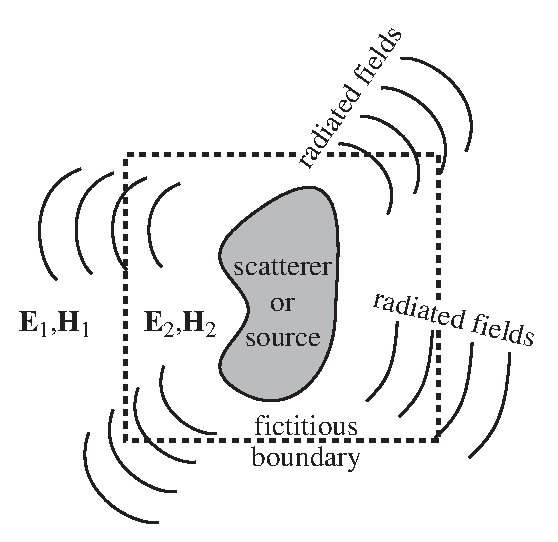
\epsfig{width=2.65in,file=Figures/Fdtd-near-to-far/radiation-cartoon.eps}\\
   (a)\\
  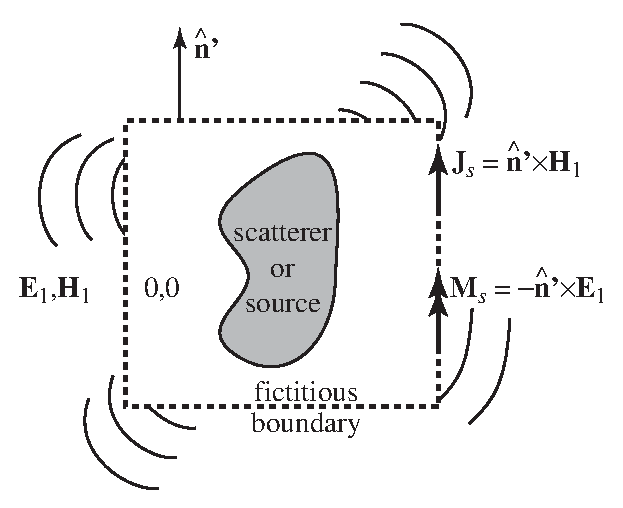
\epsfig{width=2.65in,file=Figures/Fdtd-near-to-far/radiation-cartoon-b.eps}\\
   (b)\\
  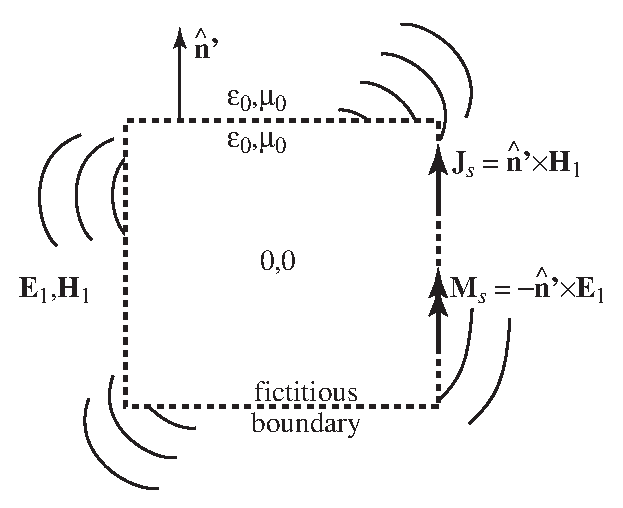
\epsfig{width=2.65in,file=Figures/Fdtd-near-to-far/radiation-cartoon-c.eps}\\
   (c)
  \end{center}
  \caption{(a) A space containing a source or scatterer that is
  surrounded by a fictitious boundary which is indicated by the dashed
  line.  The fields are continuous across this boundary.  (b) The
  fields are set to zero within the boundary.  Surface currents must
  be used to account for the discontinuity across the boundary.  (c)
  Since the fields are zero within the boundary, any inhomogeneities
  within the boundary can be discarded.}  \label{fig:equivalence}
\end{figure}

As you may recall and as will be discussed in further detail below, it
is fairly simple to find the fields radiated by a current (whether
electric or magnetic) when that current is radiating in a homogeneous
medium.  Unfortunately, as shown in Fig.\ \ref{fig:equivalence}(b),
the surface currents are not radiating in a homogeneous medium.  But,
in fact, since the fields within the fictitious boundary are zero, we
can place anything, or nothing, within the boundary and that will have
no effect on the fields exterior to the boundary.  So, let us maintain
the same surface currents but discard any inhomogeneity that were
within the boundary.  That leaves a homogeneous region as depicted in 
Fig.\ \ref{fig:equivalence}(c) and it is fairly straightforward to find
these radiated fields.

\section{Vector Potentials}

Before proceeding further, let us briefly review vector potentials.
First, consider the case (which corresponds to the physical world) where
there is no magnetic charge---electric currents can flow but magnetic
currents cannot.  Thus, 
\begin{equation}
  \nabla\cdot \Bvec_A = \nabla\cdot \mu \Hvec_A = 0 \label{eq:divBA}
\end{equation}
where the subscript $A$ indicates we are considering the case of no
magnetic charge.  There is a vector identity that the divergence of
the curl of any vector field is identically zero.  Therefore
\refeq{eq:divBA} will automatically be satisfied if we write
\begin{equation}
  \Hvec_A = \frac{1}{\mu}\nabla\times\Avec
\end{equation}
where $\Avec$ is a yet-to-be-determined field known as the magnetic
vector potential.  Now, using Faraday's law we obtain
\begin{equation}
\nabla\times\Evec_A = -j\omega\mu\Hvec_A = -j\omega\nabla\times\Avec.
\end{equation}
Using the terms on the left and the right and regrouping yields
\begin{equation}
  \nabla\times(\Evec_A + j\omega\Avec) = 0.
  \label{eq:derivingAI}
\end{equation}
The curl of the gradient of any function is identically zero.  Thus we
can set the term in parentheses equal to the (negative of the)
gradient of some unknown scalar electric potential function $\Phi_e$
and in this way \refeq{eq:derivingAI} will automatically be satisfied.
Therefore we have
\begin{equation}
  \Evec_A + j\omega\Avec = -\nabla\Phi_e
\end{equation}
or, after rearranging, 
\begin{equation}
  \Evec_A = -j\omega\Avec -\nabla\Phi_e.
\end{equation}

Using the remaining curl equation, Ampere's law, we can write
\begin{eqnarray}
\nabla\times\Hvec_A &=& \Jvec + j\omega\epsilon\Evec_A \\
\nabla\times\frac{1}{\mu}\nabla\times\Avec &=& 
  \Jvec + j\omega\epsilon(-j\omega\Avec -\nabla\Phi_e)
\end{eqnarray}
Multiplying through by $\mu$ and expanding the curl operations yields
\begin{equation}
\nabla(\nabla\cdot\Avec)-\nabla^2\Avec 
 = \mu\Jvec
   + \omega^2\mu\epsilon\Avec
   - j\omega\mu\epsilon\nabla\Phi_e.
\end{equation}
Regrouping terms yields
\begin{equation}
\nabla^2\Avec + \omega^2\mu\epsilon\Avec
 = -\mu\Jvec
   +\nabla(\nabla\cdot\Avec + j\omega\mu\epsilon\Phi_e).
 \label{eq:aVecDiffEqInitial}
\end{equation}
So far we have said what the curl of $\Avec$ must be, but that does
not fully describe the field.  To fully describe a vector field one
must specify the curl, the divergence, and the value at a point (which
we will ultimately assume is zero at a infinite distance from the
origin).  We are free to make the divergence of $\Avec$ any convenient
value.  Let us use the ``Lorentz gauge'' of
\begin{equation}
  \nabla\cdot\Avec =  -j\omega\mu\epsilon\Phi_e.
\end{equation}
By doing this, \refeq{eq:aVecDiffEqInitial} reduces to
\begin{equation}
  \nabla^2\Avec + k^2\Avec = -\mu\Jvec.
 \label{eq:aVecDiffEq}
\end{equation}
where $k=\omega\sqrt{\mu\epsilon}$.

Distinct from the scenario described above, let us imagine a situation
where there is no free electric charge.  Magnetic currents can flow,
but electric currents cannot.  Thus the divergence of the electric
flux density is
\begin{equation}
  \nabla\cdot \Dvec_F = \nabla\cdot \epsilon \Evec_F = 0 \label{eq:divDF}
\end{equation}
where here the subscript $F$ is used to indicate the case of no
electric charge.  Again, this equation will be satisfied automatically
if we represent the electric field as the curl of some potential
function $\Fvec$.  To this end we write
\begin{equation}
  \Evec_F = -\frac{1}{\epsilon}\nabla\times\Fvec
\end{equation}
where $\Fvec$ is known as the electric vector potential.  

Following steps similar to the ones we used to obtain
\refeq{eq:aVecDiffEq}, one can obtain the differential equation
that governs $\Fvec$, namely,
\begin{equation}
  \nabla^2 \Fvec + k^2 \Fvec = -\epsilon \Mvec.\label{eq:fVecDiffEq} 
\end{equation}
Thus both $\Avec$ and $\Fvec$ are governed by the wave equation.  We
see that the source of $\Avec$, i.e., the forcing function that
creates $\Avec$ is the electric current $\Jvec$.  Similarly, the
source of $\Fvec$ is the magnetic current $\Mvec$.  (We have not yet
restricted these currents to be surface currents.  At this point they
can be any current distribution, whether distributed throughout a
volume, over a surface, or along a line.)

Note that both the Laplacian ($\nabla^2$) and the constant $k^2$ that
appear in \refeq{eq:aVecDiffEq} and \refeq{eq:fVecDiffEq} are scalar
operators.  They do not change the orientation of a vector.  Thus, the
$x$ component of $\Jvec$ gives rise to the $x$ component of $\Avec$,
the $y$ component of $\Mvec$ gives rise to the $y$ component of
$\Fvec$, and so on.  In this way, \refeq{eq:aVecDiffEq} and
\refeq{eq:fVecDiffEq} could each be broken into their three
Cartesian components and we would be left with six scalar equations.

These equations have relatively straightforward solutions.  Let us
consider a slightly simplified problem, the solution of which can
easily be extended to the full general problem.  Consider the case of
an incremental current of length $d\ell$ that is located at
the origin and oriented in the $z$ direction.  In this case 
\refeq{eq:aVecDiffEq} reduces to 
\begin{equation}
  \nabla^2 A_z(\rvec) + k^2 A_z(\rvec) = -\mu I d\ell \delta(\rvec)
  \label{eq:azGoverningEq}
\end{equation}
where $I$ is the amount of current and $\delta(\rvec)$ is the 3D Dirac
delta function.  The Dirac
delta function is zero expect when its argument is zero.  For an
argument of zero, $\delta(\rvec)$ is singular, i.e., infinite.
However, this singularity is integrable.  A volume integral of any
region of space that includes the Dirac delta function at the origin
(i.e., $\rvec=0$) will yield unit volume.  For any observation point
other than the origin, \refeq{eq:azGoverningEq} can be written
\begin{equation}
  \nabla^2 A_z(\rvec) + k^2 A_z(\rvec) = 0 \qquad \rvec\neq 0.
\end{equation}
It is rather easy to show that a general solution to this is
\begin{equation}
  A_z(\rvec) = C_1\frac{e^{-jkr}}{r} +  C_2\frac{e^{jkr}}{r}.
\end{equation}
We discard the second term on the right-hand side since that
represents a spherical wave propagating in toward the origin.  Thus we
are left with
\begin{equation}
  A_z(\rvec) = C_1\frac{e^{-jkr}}{r}
\end{equation}
where we must now determine the constant $C_1$ based on the ``driving
function'' on the right side of \refeq{eq:azGoverningEq}.

To obtain $C_1$, we integrate both side of \refeq{eq:azGoverningEq}
over a small spherical volume of radius $r_0$ and take the limit as
$r_0$ approaches zero:
\begin{equation}
  \lim_{r_0\rightarrow 0} \int_V
  \left[\nabla^2 A_z + k^2 A_z\right] dv
   = 
  \lim_{r_0\rightarrow 0}
  \int_V -\mu I d\ell \delta(\rvec) dv.
\label{eq:intOfAz}
\end{equation}
Using the sifting property of the delta function, the right-hand side
of \refeq{eq:intOfAz} is simply $-\mu I d\ell$.  For the left-hand side,
we first expand the integral associated with the second term in the
square brackets
\begin{equation}
  \lim_{r_0\rightarrow 0}
  \int_{r=0}^{r_0}
  \int_{\theta=0}^{\pi}
  \int_{\phi=0}^{2\pi}
  k^2 C_1 \frac{e^{-jk r}}{r} r^2\sin\theta\,d\phi\,d\theta\,dr.
\end{equation}
Including the term $r^2\sin\theta$, which is contributed by the
volume element $dv$, the entire integrand is proportional to $r$.
Therefore as $r_0$ (the upper limit of integration in $r$) goes to
zero, this integral goes to zero.

The remaining integral on the left side of \refeq{eq:intOfAz} is
\begin{equation}
  \lim_{r_0\rightarrow 0} \int_V
  \nabla\cdot\nabla A_z dv = 
  \lim_{r_0\rightarrow 0}
  \oint_S
  \nabla A_z \cdot \mathbf{ds}
\end{equation}
where we have used the divergence theorem to convert the volume
integral to a surface integral (and used the fact that $\nabla^2 =
\nabla\cdot\nabla$).  The integrand of the surface integral is given
by
\begin{equation}
  \left.\nabla A_z\right|_{r=r_0} = 
  \left.\hat{r}\frac{\partial A_z}{\partial r}\right|_{r=r_0} =
  \hat{r}\left(-\frac{e^{-jk r_0}}{r_0^2}
             -jk\frac{e^{-jk r_0}}{r_0}\right)C_1.
\end{equation}
The surface element $\mathbf{ds}$ is given by $\hat{r}\,r_0^2 \sin\theta
d\phi\,d\theta$ so that the entire surface integral is given by
\begin{equation}
  \lim_{r_0\rightarrow 0}
  \int_{\theta=0}^{\pi}
  \int_{\phi=0}^{2\pi}
  C_1 e^{-jk r_0}(-1-jk r_0)
  \sin\theta d\phi\,d\theta =
  \lim_{r_0\rightarrow 0}
  -C_1 e^{-jk r_0}(1+jk r_0) 4 \pi = -C_1 4 \pi.
\end{equation}
Equating this with the right-hand side of \refeq{eq:azGoverningEq}, we
can solve for $C_1$.  The final result is
\begin{equation}
  C_1 = \frac{\mu I d\ell}{4 \pi}.
\end{equation}

It should be noted that there is actually nothing special about having
$r_0$ approach zero.  The same coefficient is obtained for any value
of $r_0$.  Letting $r_0$ approach zero merely simplifies the problem a
bit.

We now have that a filamentary current $I$ of length $d\ell$
located at the origin and oriented in the $z$ direction produces the
vector potential
\begin{equation}
  A_z(\rvec) = \frac{\mu I d\ell}{4 \pi}\frac{e^{-jkr}}{r}.
\end{equation}
This is simply a spherical wave radiating symmetrically away from the
origin.  If the source is located at the point $\rvec'$ instead of the
origin, one merely needs to account for this displacement.  The vector
potential in that case is
\begin{equation}
  A_z(\rvec) = \frac{\mu I d\ell}{4 \pi}
               \frac{e^{-jk|\rvec-\rvec'|}}{|\rvec-\rvec'|}.
\end{equation}
If the current was oriented in the $x$ or $y$ direction, that would
produce a vector potential that only had a $x$ or $y$ component,
respectively.  

For a current source, the ``strength'' of the source is, in one way of
thinking, determined by the amount of current that is flowing times
the length over which that current flows.  For a filament we have that
the ``source strength'' is given by $I d\ell$.  For a surface
current the equivalent concept is $J_s ds$ where $J_s$ is the
surface current density in Amperes/meter and $ds$ is an
incremental surface area.  Similarly, for a volumetric current, the 
equivalent term is $J dv$ where $J$ is the current density in
Amperes/meter$^2$ and $dv$ is an incremental volume.

Instead of having just a point source, currents can be distributed
throughout space.  To get the corresponding vector potentials, we
merely have to sum the contributions of the current wherever it
exists, accounting for the location (displacement from the origin),
the orientation, and the amount of current.

For surface currents, the vector potentials are given by
\begin{eqnarray}
\Avec(\rvec) &=&\mu \oint_S \Jvec_s(\rvec')
             \frac{e^{-jk|\rvec-\rvec'|}}{4\pi|\rvec-\rvec'|}
             ds',  \label{eq:aVecThreeD} \\
\Fvec(\rvec) &=&\epsilon \oint_S \Mvec_s(\rvec')
             \frac{e^{-jk|\rvec-\rvec'|}}{4\pi|\rvec-\rvec'|}
             ds', \label{eq:fVecThreeD} 
\end{eqnarray}
where, as before, $\rvec$ is the observation point, $\rvec'$ is the
location of the source point (i.e., the location of the currents), and
$S$ is the surface over which the current flows.

Equations \refeq{eq:aVecThreeD} and \refeq{eq:fVecThreeD} give the
vector potentials at an arbitrary observation point $\rvec$ in three
dimensions.  The surface $S$ is a surface that exists in the 3D space
(such as the surface of sphere or a cube).  

Let us consider the two-dimensional case.  We can consider the 2D case
as a special case in 3D in which there is no variation in the $z$
direction.  The observation point is a point in the $xy$ plane
specified by the vector $\rhovec$.  Thus, the magnetic vector
potential could be written as 
\begin{eqnarray}
\Avec(\rhovec) &=& \mu \oint_L\int_{z'=-\infty}^\infty
             \Jvec_s(\rhovec')
     \frac{e^{-jk\sqrt{|\rhovec-\rhovec'|^2+z'^2}}}
          {4\pi\sqrt{|\rhovec-\rhovec'|^2+z'^2}}
             dz'd\ell',\\
     &=& \mu \oint_L\Jvec_s(\rhovec')
     \left(\,\,\int_{z'=-\infty}^\infty
     \frac{e^{-jk\sqrt{|\rhovec-\rhovec'|^2+z'^2}}}
          {4\pi\sqrt{|\rhovec-\rhovec'|^2+z'^2}}
             dz'\right)d\ell'.
\end{eqnarray}
The term in parentheses can be integrated to obtain
\begin{equation}
\int_{z'=-\infty}^\infty
     \frac{e^{-jk\sqrt{|\rhovec-\rhovec'|^2+z'^2}}}
          {4\pi\sqrt{|\rhovec-\rhovec'|^2+z'^2}}
             dz' = -\frac{j}{4}H_0^{(2)}(k|\rhovec-\rhovec'|)
\end{equation}
where $H_0^{(2)}$ is the zeroth-order Hankel function of the second
kind.  This represents a cylindrical wave radiating from the point
$\rhovec'$.  Similar steps can be done for $\Fvec$ and in this way $z$
is eliminated from the expressions for the vector potentials.  We are
left with a 2D representation of the fields, namely,
\begin{eqnarray}
\Avec(\rhovec) &=& -j\frac{\mu}{4} \oint_L \Jvec(\rhovec')
             H_0^{(2)}(k|\rhovec-\rhovec'|)
             d\ell',  \label{eq:aVecTwoD} \\
\Fvec(\rhovec) &=&-j\frac{\epsilon}{4} \oint_L \Mvec(\rhovec')
             H_0^{(2)}(k|\rhovec-\rhovec'|)
             d\ell'. \label{eq:fVecTwoD} 
\end{eqnarray}
where the explicit $s$ subscript has been dropped from the currents.

The approximation of the zeroth-order Hankel function of the second
kind as the argument $\xi$ gets large is
\begin{equation}
  H_0^{(2)}(k\xi) \approx \sqrt{\frac{j 2}{\pi k\xi}}e^{-jk\xi}.
\end{equation}
Now let $\xi=|\rhovec - \rhovec'|$ where $\rho$ is large
enough that the following approximations are valid:
\begin{equation}
 \xi \approx \left\{
  \begin{array}{ll}
    \rho-\rho'\cos\psi & \mbox{for the phase}, \\
    \rho               & \mbox{for the magnitude}.
  \end{array}\right.
\end{equation}
where, referring to Fig.\ \ref{fig:ntffGeomTwoD}, $\psi$ is the angle
between the observation angle and the angle to the source point.
(Because we are taking the cosine of $\psi$, and cosine is an even
function, it doesn't matter if we define $\psi$ as $\phi-\phi'$ or
$\phi'-\phi$ but we will take $\psi$ to be $\phi - \phi'$.)  Thus the
Hankel function can be written
\begin{equation}
  H_0^{(2)}(k|\rhovec - \rhovec'|) \approx
      \sqrt{\frac{j 2}{\pi k\rho}}e^{-jk\rho}e^{jk\rho'\cos\psi}.
\end{equation}
The $\mathbf{A}$ vector potential for a 2D problem can thus be written
\begin{eqnarray}
  \mathbf{A}(\rhovec) &=&
    -j\frac{\mu}{4}\oint_L \mathbf{J}(\rhovec')
                           H_0^{(2)}(k|\rhovec - \rhovec'|)d\ell', \\
  &\approx&
    -j\frac{\mu}{4}\sqrt{\frac{j 2}{\pi k\rho}}e^{-jk\rho}
                   \oint_L \mathbf{J}(\rhovec')
                          e^{jk\rho'\cos\psi} d\ell', \\
  &=&
    -j\frac{\mu}{4}\sqrt{\frac{j 2}{\pi k\rho}}e^{-jk\rho}
                   \mathbf{N}_{2D},
   \label{eq:afar}
\end{eqnarray}
where
\begin{equation}
  \mathbf{N}_{2D} = 
    \oint_L \mathbf{J}(\rhovec') e^{jk\rho'\cos\psi} d\ell'.
\end{equation}
Correspondingly, the $\mathbf{F}$ vector potential can be written
\begin{eqnarray}
  \mathbf{F}(\rhovec) &=&
    -j\frac{\epsilon}{4}\oint_L \mathbf{M}(\rhovec')
                           H_0^{(2)}(k|\rhovec - \rhovec'|)d\ell', \\
  &\approx&
    -j\frac{\epsilon}{4}\sqrt{\frac{j 2}{\pi k\rho}}e^{-jk\rho}
                   \oint_L \mathbf{M}(\rhovec')
                          e^{jk\rho'\cos\psi} d\ell', \\
  &=&
    -j\frac{\epsilon}{4}\sqrt{\frac{j 2}{\pi k\rho}}e^{-jk\rho}
                   \mathbf{L}_{2D},
   \label{eq:ffar}
\end{eqnarray}
where
\begin{equation}
  \mathbf{L}_{2D} = 
     \oint_L \mathbf{M}(\rhovec') e^{jk\rho'\cos\psi} d\ell'.
\end{equation}
Nominally $\mathbf{N}_{2D}$ and $\mathbf{L}_{2D}$ are functions of
$\rhovec$.  However, within these functions the only thing that
depends on $\rhovec$ is $\psi$.  The angle $\psi$ only changes for
large changes in $\rhovec$---incremental changes of $\rhovec$ will not
affect $\psi$.  Thus, derivatives of $\mathbf{N}_{2D}$ or
$\mathbf{L}_{2D}$ with respect to $\rho$, $\phi$, or $z$ (i.e.,
derivatives with respect to the unprimed coordinates) are zero.
The geometry is depicted in Fig.\ \ref{fig:ntffGeomTwoD}.

\begin{figure}
  \begin{center}
  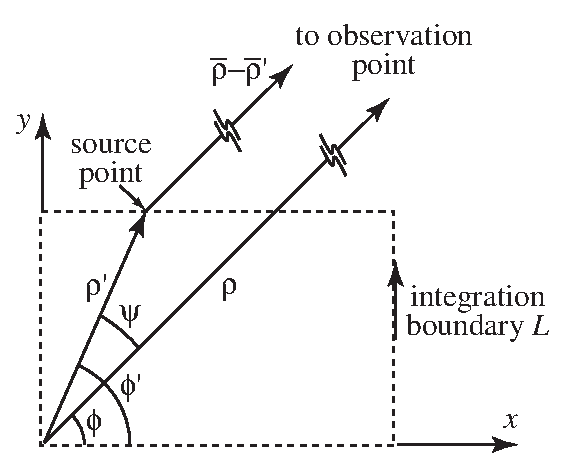
\epsfig{width=3.0in,file=Figures/Fdtd-near-to-far/ntff-2d-geometry.eps}
  \end{center}
  \caption{Geometry associated with the near-to-far-field
  transformation in 2D.}  \label{fig:ntffGeomTwoD}
\end{figure}


It is convenient to think of the currents, and subsequently
$\mathbf{N}_{2D}$ and $\mathbf{L}_{2D}$ (and ultimately the
potentials), in terms of cylindrical coordinates, i.e.,
\begin{eqnarray}
  \mathbf{J}(\rhovec) &=& J_\rho \unitvec{\rho} + 
                        J_\phi \unitvec{\phi} + 
                        J_z \zunit, \\
  \mathbf{M}(\rhovec) &=& M_\rho \unitvec{\rho} + 
                        M_\phi \unitvec{\phi} + 
                        M_z \zunit.
\end{eqnarray}

Combining the contributions from both $\Avec$ and $\Fvec$, the
electric and magnetic fields are given by
\begin{eqnarray}
  \mathbf{E}(\rhovec) &=&
    -j\omega\left[\mathbf{A} +
                  \frac{1}{k^2}\nabla(\nabla\cdot\mathbf{A})\right]
    -\frac{1}{\epsilon}\nabla\times\mathbf{F}, \label{eq:eFieldFar}
  \\
  \mathbf{H}(\rhovec) &=&
    -j\omega\left[\mathbf{F} +
                  \frac{1}{k^2}\nabla(\nabla\cdot\mathbf{F})\right]
    +\frac{1}{\mu}\nabla\times\mathbf{A}. \label{eq:hFieldFar}
\end{eqnarray}

By plugging \refeq{eq:afar} and \refeq{eq:ffar} into
\refeq{eq:eFieldFar} and \refeq{eq:hFieldFar} and performing the various
operations in cylindrical coordinates and discarding any terms that
fall off faster than $1/\sqrt{\rho}$, one can obtain expressions for
the electric and magnetic fields in the far field.  (Note that the
$\nabla$ operator acts on the unprimed coordinates and, as mentioned
above, $\mathbf{N}_{2D}$ and $\mathbf{L}_{2D}$ are not considered
functions of the unprimed coordinates.)

\section{Electric Field in the Far-Field}

Following the steps outlined in the previous section, the scattered
electric field $\Evec^s$ at the far-field point $\rhovec$ can be
obtained from the scattered ``near'' fields using
\begin{equation}
  \Evec^s(\rhovec) =
  \sqrt{\frac{j}{8\pi k}} \frac{e^{-jk\rho}}{\sqrt{\rho}} 
  \left\{\unitvec{\phi}\left(\omega\mu_0\Ntwod\cdot\unitvec{\phi}
	                     +k\Ltwod\cdot\zunit\right)
       - \zunit\left(\omega\mu_0\Ntwod\cdot\zunit
	                     -k\Ltwod\cdot\unitvec{\phi}\right)
  \right\},
\label{eq:esfar}
\end{equation}
where, as stated previously,
\begin{eqnarray}
  \Ntwod &=& 
    \oint_L \Jvec(\rhovec') e^{jk\rho'\cos\psi} d\ell', \\
  \Ltwod &=& 
    \oint_L \Mvec(\rhovec') e^{jk\rho'\cos\psi} d\ell',
\end{eqnarray}
$L$ is the closed path of integration, $\psi$, given by $\phi-\phi'$,
is the angle between the source point and observation point, $\Mvec =
-\nunit\times\Evec$, $\Jvec = \nunit\times\Hvec$, and
$\nunit$ is a unit vector normal to the integration contour on
the same side of the contour as the observation point (i.e., the
outward normal).  Unprimed coordinates correspond to the observation
point while primed coordinates indicate the ``source'' location (i.e.,
points along the contour).

Let us now restrict consideration to TM$^z$ polarization where the
non-zero field are $H_x$, $H_y$, and $E_z$.  Since the outward normal
is restricted to exist in the $xy$ plane, $\nunit\times\Hvec$ only has
a non-zero component in the $z$ direction while $-\nunit\times\Evec$
only has non-zero components in the $xy$ plane.  Thus, for this
polarization only the $z$ component of the electric field is
non-zero---the $\phi$ component of \refeq{eq:esfar} is zero.  The
electric field can be written
\begin{equation}
  E^s_z(\rhovec) =
  -\sqrt{\frac{j}{8\pi k}} \frac{e^{-jk\rho}}{\sqrt{\rho}} 
  \oint_L
  \left(\omega\mu_0\Jvec(\rhovec')\cdot\zunit
	                     -k\Mvec(\rhovec')\cdot\unitvec{\phi}\right)
  e^{jk\rho'\cos\psi} d\ell'.
\label{eq:ezfar}
\end{equation}


Usually the scattering width is of more interest than the field
itself.  For TM$^z$ polarization the two-dimensional scattering width
is defined to be
\begin{equation}
\stwo(\phi) = \lim_{|\rhovec-\rhovec'|\rightarrow\infty} 2\pi \rho
\frac{|E^s_z(\rhovec)|^2}{|E^i_z|^2} \label{eq:swidth}
\end{equation}
Noting that $\omega\mu_0=k\eta_0$ and plugging \refeq{eq:ezfar} into
\refeq{eq:swidth} and normalizing by the wavelength yields
\begin{equation}
\frac{\stwo(\phi)}{\lambda} = \frac{1}{8\pi|E^i_z|^2}
\left|\oint_{L}\left\{\eta_0\Jvec(\rhovec')\cdot\zunit
  - \Mvec(\rhovec')\cdot\unitvec{\phi}\right\}
  e^{jkr'\cos(\phi-\phi')}kd\ell'\right|^2.
\label{eq:stwo}
\end{equation}
The term $r'\cos(\phi-\phi')$ which appears in the
exponent can be written as $\runit\cdot\rhovec = \runit\cdot(x'\xunit
+ y'\yunit) = x'\cos\phi + y'\sin\phi$.  This last form is especially
useful since $\phi$ is fixed by the observation direction and
therefore the sine and cosine functions can be determined outside of
any loop (rather than over and over again as we move along the
integration contour).

For TM$^z$ polarization the unit vector normal to the integration
path is restricted to lie in the $xy$ plane, i.e., $\nunit = n'_x\xunit
+ n'_y\yunit$ where $({n'}_x^2+{n'}_y^2)^{1/2}=1$.  Thus, the electric
current $\Jvec$ is given by
\begin{equation}
  \Jvec = \nunit\times\Hvec =
  \left|
    \begin{array}{ccc}
     \xunit & \yunit & \zunit \\
     n'_x   & n'_y   & 0 \\
     H_x    & H_y    & 0
    \end{array}
  \right|
  = \zunit(n'_x H_y - n'_y H_x).
\end{equation}
The dot product of $\zunit$ and $\Jvec$ yields
\begin{equation}
  \Jvec \cdot \zunit = 
  n'_x H_y - n'_y H_x.
  \label{eq:jvecDotZ}
\end{equation}
The magnetic current is given by 
\begin{equation}
  \Mvec = -\nunit\times\Evec =
  \left|
    \begin{array}{ccc}
     \xunit & \yunit & \zunit \\
     n'_x   & n'_y   & 0 \\
     0      & 0      & E_z
    \end{array}
  \right|
  = -(\xunit n'_y E_z - \yunit n'_x E_z)
\end{equation}
The dot product of $\unitvec{\phi}$ and $\Mvec$ yields
\begin{equation}
  \Mvec\cdot\unitvec{\phi} = 
    -\xunit\cdot\unitvec{\phi} n'_y E_z +
     \yunit\cdot\unitvec{\phi} n'_x E_z =
    (n'_y \sin\phi + n'_x \cos\phi) E_z
  \label{eq:mvecDotPhi}
\end{equation}

Incorporating \refeq{eq:jvecDotZ} and \refeq{eq:mvecDotPhi} into
\refeq{eq:stwo} yields a general expression for the scattering width:
\begin{equation}
\frac{\stwo(\phi)}{\lambda} = \frac{1}{8\pi|E^i_z|^2}
\left|\oint_{L}\left\{\eta_0(n'_x H_y - n'_y H_x)
  - (n'_y \sin\phi + n'_x \cos\phi) E_z\right\}
  e^{jkr'\cos(\phi-\phi')}kd\ell'\right|^2.
\label{eq:stwoGeneral}
\end{equation}
We now want to specialize this equation to a rectangular box which is
typical of the integration boundary which would be employed in an FDTD simulation.

Assume the integration boundary corresponds to the dashed box shown
in Fig.\ \ref{fig:nfftBoundary}.
\begin{figure}
\begin{center}
\setlength{\unitlength}{2pt}
\begin{picture}(220,110)(-25,-10)
% axes
\put(-10,0){\vector(1,0){200}}
\put(182,-6){$x=m'\Delx$}
\put(0,-5){\vector(0,1){100}}
\put(-5,96){$y=n'\Dely$}
% integration boundary
\put(.5,.5){\dashbox(180,90)}
\put(2,4){$(0,0)$}
\put(155,4){$(L_x\Delx,0)$}
\put(144.5,84){$(L_x\Delx,L_y\Dely)$}
\put(2,84){$(0,L_y\Dely)$}
% side 1
\put(80,4){Side $L_4$}
\put(90,0){\vector(0,-1){9}}
\put(92,-6){$\nunit=-\yunit$}
% side 2
\put(160,43){Side $L_3$}
\put(180,45){\vector(1,0){9}}
\put(182,47){$\nunit=\xunit$}
% side 3
\put(80,84){Side $L_2$}
\put(90,90){\vector(0,1){9}}
\put(92,95){$\nunit=\yunit$}
% side 2
\put(2,43){Side $L_1$}
\put(0,45){\vector(-1,0){9}}
\put(-25,47){$\nunit=-\xunit$}
\end{picture}
\end{center}
\caption{Depiction of integration boundary for near-to-far-field
transformation in the FDTD grid. \label{fig:nfftBoundary}}
\end{figure}
The width of this rectangle is $L_x\Delx$ and the height is
$L_y\Dely$.  In an FDTD grid there are $L_x+1$ samples of the fields
along the top and bottom (i.e., spanning the width) and $L_y+1$ total
samples along the left and right (i.e., spanning the height).  The
integration over the closed path $L$ consists of the integration over
the four sides of this box, i.e., $L = L_1 + L_2 + L_3 + L_4$.  Using
this geometry, the quantities needed to perform each integral are
presented in the following two tables.

\begin{center}
\begin{tabular}{c|l|l|r|r}
   & \multicolumn{2}{c|}{$\nunit$}
   & $\Jvec\cdot\zunit$  
   & \multicolumn{1}{c}{$\Mvec\cdot\unitvec{\phi}$}
\\ \hline
Side $L_1$ \rule[-7pt]{0pt}{20pt}
   & $n'_x=-1$ & $n'_y=0$
   & $-H_y$
   & $-\cos\phi E_z$
 \\\hline
Side $L_2$ \rule[-7pt]{0pt}{20pt}
   & $n'_x=0$ & $n'_y=1$
   & $-H_x$
   & $\sin\phi E_z$
\\\hline
Side $L_3$ \rule[-7pt]{0pt}{20pt}
   & $n'_x=1$ & $n'_y=0$ 
   & $H_y$
   & $\cos\phi E_z$
\\\hline
Side $L_4$ \rule[-7pt]{0pt}{20pt}
   & $n'_x=0$ & $n'_y=-1$
   & $H_x$
   & $-\sin\phi E_z$ 
\end{tabular}
\end{center}

\begin{center}
\begin{tabular}{c|c|c|c}
   & $\phi'$  & $\rho'$ & $\unitvec{\rho}\cdot\rhovec'$
\\ \hline
Side $L_1$ \rule[-7pt]{0pt}{20pt}
   & $\pi/2$
   & $n'\Dely$
   & $n'  \Dely \sin\phi$
\\\hline
Side $L_2$ \rule[-7pt]{0pt}{20pt}
   & $\tan^{-1}(L_y/m')$
   & $\sqrt{(m'\Delx)^2+(L_y\Dely)^2}$
   & $m'  \Delx \cos\phi + L_y \Dely \sin\phi$
\\\hline
Side $L_3$ \rule[-7pt]{0pt}{20pt}
   & $\tan^{-1}(n'/L_x)$
   & $\sqrt{(L_x\Delx)^2+(n'\Dely)^2}$
   & $L_x \Delx \cos\phi + n'  \Dely \sin\phi$
\\\hline
Side $L_4$ \rule[-7pt]{0pt}{20pt}
   & $0$ 
   & $m' \Delx \cos\phi$
   & $m'\Dely$
\end{tabular}
\end{center}
Note that in the second table the value $n'$ represents the
vertical displacement along Side $L_1$ or $L_3$.  It varies between
$0$ and $L_y$ and should not be confused with the outward normal
$\nunit$ and its components $n_x'$ and $n_y'$.

Assume that the spatial step sizes are equal so that
$\Delx=\Dely=\delta$.  Further assume that the problem has be
discretized using $\ppw$ points per wavelength so that the wavenumber
can be written $k=2\pi/\lambda=2\pi/(\ppw\delta)$.  Combining all
together, the scattering width is given by
\begin{eqnarray}
\frac{\stwo(\phi)}{\lambda} &=& \frac{1}{8\pi|E^i_z|^2}
\left|\,\,
\int^{L_x}_{m'=0}
% side 4
\left\{\left[\eta_0 H_x(m',0) + \sin\phi E_z(m',0)\right]
  e^{j\frac{2\pi}{\ppw}m'\cos\phi}\right.\right.  \nonumber\\
&&
\mbox{\hspace{.48in}} -
% side 2
\left.\left[\eta_0 H_x(m',L_y) + \sin\phi E_z(m',L_y)\right]
  e^{j\frac{2\pi}{\ppw}(m'\cos\phi + L_y\sin\phi)}
  \right\}\frac{2\pi}{\ppw}dm' \nonumber\\ 
&&\mbox{\hspace{.13in}} +
% side 1
\left.\int^{L_y}_{n'=0}
\left\{-\left[\eta_0 H_y(0,n') - \cos\phi E_z(0,n')\right]
  e^{j\frac{2\pi}{\ppw}n'\sin\phi}
  \right.\right. \nonumber\\
&&
\mbox{\hspace{.48in}} +
% side 3
\left.\left.\left[\eta_0 H_y(L_x,n') - \cos\phi E_z(L_x,n')\right]
  e^{j\frac{2\pi}{\ppw}(L_x\cos\phi+n'\sin\phi)}\right\}
  \frac{2\pi}{\ppw}dn'\right|^2\,\,\,\mbox{}
\label{eq:sall}
\end{eqnarray}
Again we note that the integration variable for the second integral is
$n'$ which corresponds to displacement along the vertical sides.  The
fields in this expression are phasor (frequency-domain) quantities and
hence are complex.  Although this equation may look rather messy, as
described in the next two sections, the phasors can be obtained rather
simply with a running DFT and the integration can be calculated with a
sum.

Because of the staggered nature of the FDTD grid, the electric and
magnetic fields will not be collocated on the integration
boundary---they will be offset in both space and time.  A spatial
average of either the electric or magnetic field will have to be
performed to obtain the fields at the proper location.  In the past, a
simple arithmetic average was typically used to account for the
spatial offsets.  However, as will discussed, one can do better by
using a harmonic average in space.  For the temporal offset, a simple
phase correction can be used to collocate the fields in time.


\section{Simpson's Composite Integration}

Assume we wish to integrate the function $f(x)$ over the interval
$0\leq x\leq L$ where $L$ is an even integer.  The integral can be
obtained using Simpson's composite integration as follows
\begin{equation}
\int_0^L f(x) dx \approx
\frac{1}{3}\left[
f(0) + 2\sum_{m=1}^{L/2-1}f(2m) + 4\sum_{m=1}^{L/2}f(2m-1) + f(L)
\right]
\end{equation}
Note that this approximation requires a total of $L+1$ samples of the
function (so we need an odd number of samples).  Using Simpson's
approximation yields quite a bit of additional accuracy over what
would be obtained using a straight Riemann sum and it costs
essentially nothing (it just requires slightly more bookkeeping).

%===================================================================

\section{Collocating the Electric and Magnetic Fields: The Geometric
Mean}

Figure \ref{fig:geometryNTFF} depicts an integration boundary in a
TM$^z$ grid.
\begin{figure}
\begin{center}
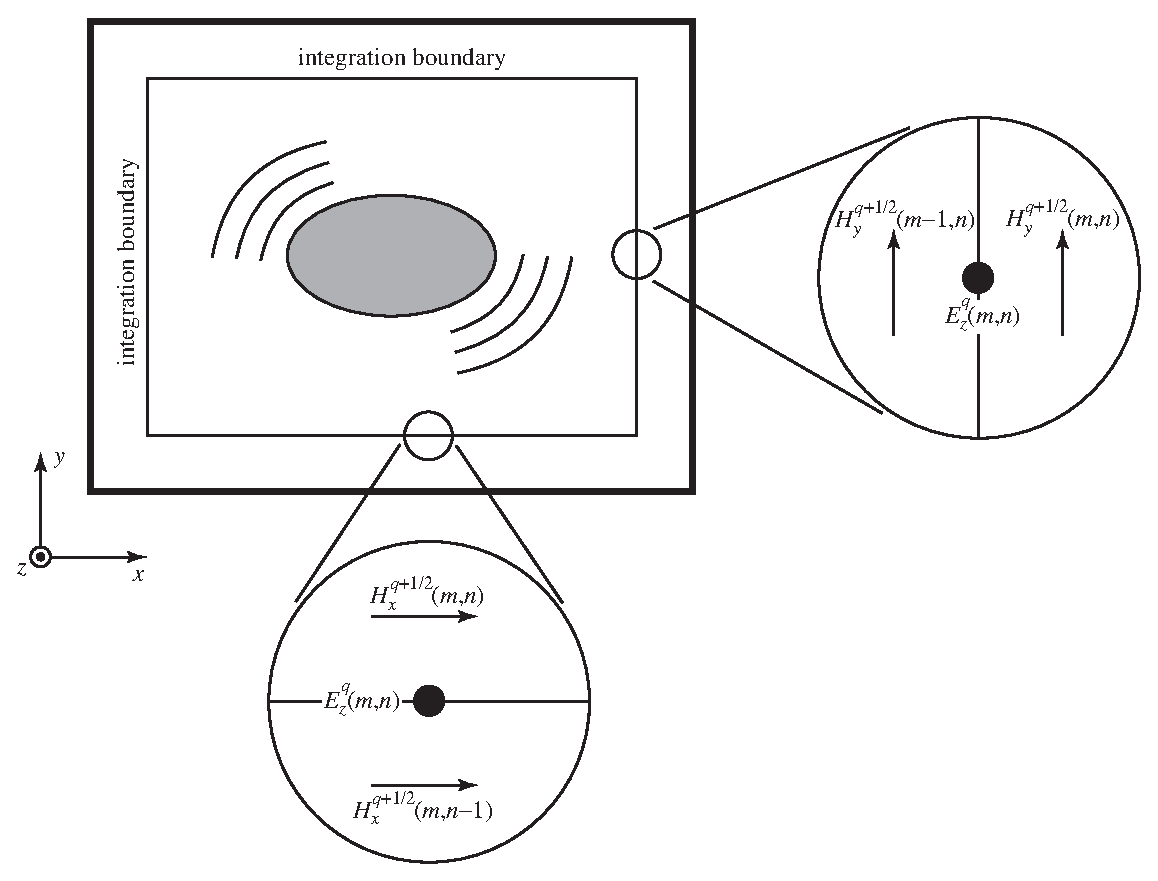
\epsfig{width=4in,file=Figures/Fdtd-near-to-far/geometryNTFF.eps}
\vspace{-.1in}
\end{center}
\caption{Depiction of a TM$^z$ grid showing the integration boundary.
The boundary is assumed to be aligned with electric-field nodes.  The
expanded views show the offset of the magnetic-field nodes from the
boundary.}
\label{fig:geometryNTFF}
\end{figure}
The boundary is assumed to be aligned with the electric-field nodes,
i.e., the $E_z$ nodes.  The expanded views show a portion of the
boundary along the right side and the bottom.  The field notation
employs superscripts to indicate time steps while spatial indices are
given as arguments within parentheses.  Half-step spatial offsets are
implicitly understood.  Thus, the nodes in space-time and the
corresponding notation are
\begin{eqnarray}
H_x^{(q-1/2)\Delt}(m\Delx,[n+1/2]\Dely) &=&
  H_x^{q-1/2}(m,n), \\
H_y^{(q-1/2)\Delt}([m+1/2]\Delx,n\Dely) &=&
  H_y^{q-1/2}(m,n), \\
E_z^{q\Delt}(m\Delx,n\Dely) &=&
  E_z^{q}(m,n),
\end{eqnarray}
where $\Delx$ and $\Dely$ are the spatial steps in the $x$ and
$y$ directions, respectively, and $\Delt$ is the temporal step.
The index $q$ indicates the temporal step and we assume it varies
between $1$ and $N_T$ which is the total number of time-steps.

Near-to-far-field (NTFF) transforms require that the fields be defined
over a single surface and use the same phase reference.  For harmonic
fields, the temporal offset can be easily accounted for with a phase
factor.  Assume the magnetic fields have been recorded at times of
$q=1/2, 3/2, 5/2,\ldots$ while the electric field has been recorded at
times of $q=1, 2, 3,\ldots$\@ For the harmonic transforms of interest
here, the time-domain near-fields are Fourier transformed to the
frequency domain.  For example, the harmonic electric field on the
boundary is given by
\begin{eqnarray}
  \hat{E}^k_z(m,n)
    &=& {\cal F}\left[E_z^q(m,n)\right], \\
    &=& \frac{1}{N_T}
        \sum_{q=\langle N_T\rangle} E_z^q(m,n) e^{-jk\frac{2\pi}{N_T}q}.
        \label{eq:dft}
\end{eqnarray}
where $\cal F$ is the discrete Fourier transform.  For situations
where the entire spectrum is not of interest, typically a running
discrete Fourier transform will be used only at the particular
frequencies of interest.  A frequency is specified by the index $k$
which varies between zero (dc) and $N_T-1$.  Regardless of the
implementation used, the resulting spectral terms $\hat{E}^k_z$ will be
the same.

The time-domain series $E_z^q(m,n)$ can be obtained from
$\hat{E}^k_z(m,n)$ via
\begin{equation}
  E_z^q(m,n) = \sum_{k=\langle N_T\rangle} 
               \hat{E}^k_z(m,n) e^{jk\frac{2\pi}{N_T}q}.
  \label{eq:ezq}
\end{equation}
Because of the temporal offset between the electric and magnetic
fields, the desired field is actually $E_z^{q-1/2}(m,n)$, thus,
plugging $q-1/2$ into \refeq{eq:ezq} yields
\begin{equation}
  E_z^{q-1/2}(m,n) =
  \sum_{k=\langle N_T\rangle}
  \left(\hat{E}^k_z(m,n)e^{-jk\frac{\pi}{N_T}}\right) 
                        e^{jk\frac{2\pi}{N_T}q}.
\end{equation}
In practice one calculates $\hat{E}^k_z(m,n)$ and the spectral
representation of the magnetic fields in the same way, i.e., as in
\refeq{eq:dft}.  Then one multiplies $\hat{E}^k_z(m,n)$ by
$\exp(-jk\pi/N_T)$ to account for the temporal offset.

The spatial offset is slightly more problematic than the temporal
offset.  As shown in Fig.\ \ref{fig:geometryNTFF}, the integration
boundary can be aligned with only one of the fields.  The magnetic
field tangential to the integration boundary is found from the nodes
that are a spatial half-step to either side of the boundary.

To obtain the magnetic field on the boundary, the traditional approach
has been to use a spatial average of the nodes to either side of the
boundary.  For example, along the right side of the boundary, the
harmonic magnetic field would be given by
\begin{equation}
  \hat{H}^k_y(m,n) = 
  \frac{1}{2}{\cal F}\left[H_y^{q-1/2}(m-1,n)+H_y^{q-1/2}(m,n)\right].
  \label{eq:arithmetic}
\end{equation}
Because of this spatial average, $\hat{H}_y(m,n)$ and $\hat{E}_z(m,n)$
are assumed to be collocated and, with the temporal phase correction,
can be used to determine the equivalent currents over the integration
boundary (which are then used in the NTFF transform itself).

Unfortunately the arithmetic mean used in \refeq{eq:arithmetic}
introduces errors.  To illustrate this, assume a harmonic plane wave
is propagating in the grid.  The temporal frequency $\omega$ is $2\pi
k'/N_T$ where $k'$ is an integer constant and, as before, $N_T$ is the
total number of time-steps in a simulation.  The $y$ component of the
magnetic field is given by
\begin{eqnarray}
   \lefteqn{H_y^{q-1/2}(m,n) =
     \cos\left(\omega\left[q-\half\right]\Delt-\xi\right)}, \\
   &=&\!\!\!\!
      \frac{e^{j\left(k'\frac{2\pi}{N_T}[q-\half]\Delt+\xi\right)}+
            e^{-j\left(k'\frac{2\pi}{N_T}[q-\half]\Delt+\xi\right)}}{2},
   \label{eq:hyPlaneWave}
\end{eqnarray}
where $\xi=\beta_x(m+1/2)\Delx + \beta_y n\Dely$, and $\beta_x$ and
$\beta_y$ are the $x$ and $y$ components of the wave vector,
respectively.  Taking the discrete Fourier transform of
\refeq{eq:hyPlaneWave}, i.e.,
\begin{equation}
  \hat{H}^k_y(m,n)
    = \frac{1}{N_T}
        \sum_{q=\langle N_T\rangle} H_y^{q-1/2}(m,n) 
             e^{-jk\frac{2\pi}{N_T}\left(q-\half\right)},
\end{equation}
one notes that the sum yields zero when $k$ is anything other than
$k'$ or $N_T-k'$.  The values of $k$ that yield non-zero correspond
to the positive and negative frequency of the continuous world and,
like the continuous world, the corresponding spectral values are
complex conjugates.  Without loss of generality, we will continue the
discussion in terms of the spectral component corresponding to the
positive frequency, i.e., 
\begin{equation}
  \hat{H}^{k'}_y(m,n) =
    \half \exp(-j[\beta_x(m+1/2)\Delx + \beta_y n\Dely]).
\end{equation}
(Note that since the time-domain functions are real-valued, in
practice one does not need to calculate the transform at any of the
negative frequencies.  They are merely the complex conjugates of the
values at the positive frequencies.)

Because the Fourier transform is a linear operator, using
\refeq{eq:hyPlaneWave} in \refeq{eq:arithmetic} yields
\begin{eqnarray}
 \hspace{-.15in} 
  \hat{H}^{k'}_y(m,n) \!\!\!\!\!&=&\!\!\!\!
   e^{-j\beta_y n\Dely}
   \frac{e^{-j\beta_x\!\left(m-\frac{1}{2}\right)\!\Delx} + 
         e^{-j\beta_x\!\left(m+\frac{1}{2}\right)\!\Delx}}{4}, \\
   &=&\!\!\!\!
   \half e^{-j(\beta_x m \Delx + \beta_y n\Dely)} 
   \cos\!\left(\frac{\beta_x\Delx}{2}\right).
   \label{eq:arithmeticPlane}
\end{eqnarray}
The exact expression for the magnetic field on the integration
boundary is $\exp(-j[\beta_x m \Delx + \beta_y n\Dely])/2$.  Thus, the
cosine term represents an error---one which vanishes only in the limit
as the spatial-step size goes to zero.

Instead of taking the Fourier transform of the average of the
time-domain fields, let us take the Fourier transform of the fields to
either side of the boundary.  We define the transforms as
\begin{eqnarray}
  \hat{H}^+_y(m,n) &=& 
    {\cal F}\!\left[H_y^{q-1/2}(m,n)\right], \\
  \hat{H}^-_y(m,n) &=& 
    {\cal F}\!\left[H_y^{q-1/2}(m-1,n)\right].
\end{eqnarray}
Still assuming a single harmonic plane wave, for the ``positive
frequency'' corresponding to $k=k'$, $\hat{H}^+_y(m,n)$ and
$\hat{H}^-_y(m,n)$ are given by
\begin{eqnarray}
  \hat{H}^+_y(m,n) &=& 
    \half e^{-j(\beta_x(m+1/2)\Delx + \beta_y n\Dely)}, \\
  \hat{H}^-_y(m,n) &=& 
    \half e^{-j(\beta_x(m-1/2)\Delx + \beta_y n\Dely)}.
\end{eqnarray}
Were one to calculate the arithmetic mean of $\hat{H}^+_y(m,n)$ and
$\hat{H}^-_y(m,n)$, the result would be the same as given in
\refeq{eq:arithmeticPlane}.  However, consider the geometric mean
(where the geometric mean of $a$ and $b$ is $\sqrt{ab}$) of 
$\hat{H}^+_y(m,n)$ and
$\hat{H}^-_y(m,n)$:
\begin{eqnarray}
  \hat{H}^{k'}_y(m,n) &=&
    \left(\hat{H}^+_y(m,n)\hat{H}^-_y(m,n)\right)^{1/2}, \\
  &=&  
    \half e^{-j(\beta_x m\Delx + \beta_y n\Dely)}.
\end{eqnarray}
This is precisely the correct answer.  There is no error introduced by
the geometric mean.  A note of caution: when calculating the square
root of these complex quantities, one must ensure that the proper
branch cut is selected.  Thus, when $\hat{H}^+_y(m,n)$ and
$\hat{H}^-_y(m,n)$ have phases near $\pm\pi$ the geometric mean should
also have a phase near $\pm\pi$ rather than near zero.

In practice, at any given frequency there will be an angular spectrum
of wave vectors present and hence any averaging, whether geometric or
arithmetic, will introduce some errors.  However, for a single wave
vector the geometric mean is exact and it has been our experience that
the geometric mean provides superior results for nearly all
discretizations and scattering angles.  The following section
demonstration the use of the geometric mean in several scenarios.

%%%%%%%%%%%%%%%%%%%%%%%%%%%%%%%%%%%%%%%%%%%%%%%%%%%%%%%%%%%%%%%%%%%%%%%
%%%%%%%%%%%%%%%%%%%%%%%%%%%%%%%%%%%%%%%%%%%%%%%%%%%%%%%%%%%%%%%%%%%%%%%
%%%%%%%%%%%%%%%%%%%%%%%%%%%%%%%%%%%%%%%%%%%%%%%%%%%%%%%%%%%%%%%%%%%%%%%
\section{NTFF Transformations Using the Geometric Mean
\label{sec:gmNtffResults}}

\subsection{Double-Slit Radiation}

To demonstrate the difference between the arithmetic and geometric
mean, we begin by considering the radiation from a double-slit
aperture in a perfect electrical-conductor (PEC) screen which is
illuminated by a normally incident pulsed plane wave.  TM$^z$
polarization is assumed.  As shown in Fig.\
\ref{fig:youngGeometry}(a), in this case the boundary over which the
fields are measured is three-sided and exists on only one side of the
screen.

Given the fields over the three-sided boundary, one then assumes the
fields ``interior'' to this boundary (i.e., the region which includes
the slits) are zero while the fields exterior to the boundary are
unchanged.  To account for the discontinuity in the fields across the
integration boundary, surface currents must be present.  Since the
fields are zero within the boundary, one can replace the actual
interior with anything without affecting the exterior fields.  One
thus assumes that the slits are not present---that the PEC plane is
unbroken.  The surface currents over the three-sided boundary are now
radiating in the presence of an infinite plane.  The far-field
radiation can be calculated with a three-sided integral where one uses
the Green's function for a source above an infinite plane.  This,
equivalently, from image theory, is simply the radiation from the
original (measured) current and the image of the current.  Both the
measured current and the image current are radiating in free space.
In this way the three-sided boundary can be replaced with a closed
four-sided boundary as shown in Fig.\ \ref{fig:youngGeometry}(b).  The
corresponding currents over this surface, i.e., the measured currents
over half the boundary and the image currents over the other half, are
transformed to the far field.  

The incident field is introduced over a total-field/scattered-field
(TFSF) boundary which only exists to the left side of the screen.  The
grid is terminated with an eight-cell perfectly matched layer (PML).
\begin{figure}
\begin{center}
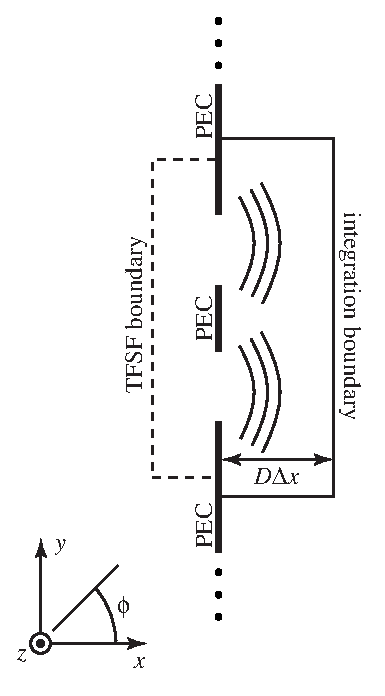
\epsfig{width=1.8in,file=Figures/Fdtd-near-to-far/youngGeomtry.eps}\\
\vspace{-.15in}
(a)\\
\vspace{.15in}
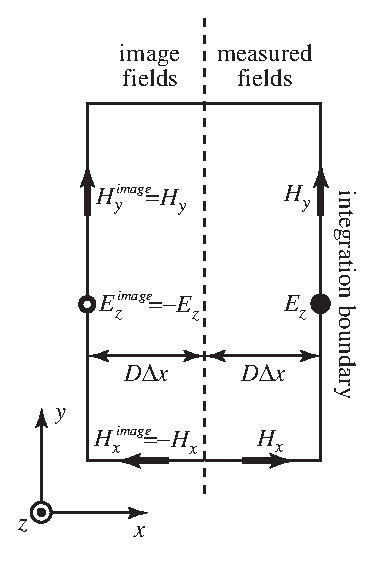
\epsfig{width=1.8in,file=Figures/Fdtd-near-to-far/imageFields.eps}\\
\vspace{-.15in}
(b)
\end{center}
\caption{(a) Geometry of the double-slit experiment.  A pulsed plane
wave is introduced via a TFSF boundary on the left side of the screen.
The field are recorded over the three-sided integration boundary to
the left of the screen.  (b) Image theory is used to create a
four-sided closed surface over which the currents are transformed
to the far-field.  The dashed line corresponds to the location where
the PEC plane had been.}
\label{fig:youngGeometry}
\end{figure}

The right side of the integration surface is $D$ cells away from the
PEC screen.  The length of the right side of the integration boundary
is held fixed at $75$ cells.  In principle, the location of the
integration boundary should make no difference to the far-fields.
However, when using the arithmetic mean, the far-fields are sensitive
to the boundary location, i.e., sensitive to the value of $D$.  Note
that were a single component of the field integrated over the
aperture, as advocated by \cite{sullivan2001a}, averaging is not an
issue.  However, that approach is restricted to screens which are
planar and there are no inhomogeneities present other than the screen.
The approach we advocate can accommodate any screen or scatterer
geometry provided it can be contained within the integration boundary.
Nevertheless, we will employ the aperture-based approach as a
reference solution.

The simulation uses ``slits'' which are $15$ cells wide.  The PEC
between the slits is $30$ cells wide.  The excitation is a Ricker
wavelet discretized such that there are $30$ cells per wavelength at
the most energetic frequency.  The simulation is run at the $2$D Courant
limit ($1/\sqrt{2}$) for $1024$ time steps.  

Figure \ref{fig:youngArithmetic}(a) shows the far-field radiation
pattern which is obtained using the arithmetic mean.  The pattern is
symmetric about zero degrees which corresponds to the direction normal
to the screen.  The radiation pattern is calculated using
\begin{equation}
  \frac{1}{\lambda}\lim_{\rho\rightarrow\infty}
   \left[2\pi\rho\frac{|\hat{E}_z(\phi)|^2}{|\hat{E}_z^i|^2}\right]
  \label{eq:radPattern}
\end{equation}
where $\phi$ is the scattering angle, $\rho$ is the distance from the
slits, $\hat{E}_z(\phi)$ is the field radiated in the $\phi$
direction, and $\hat{E}_z^i$ is the complex amplitude of the incident
plane wave at the frequency of interest.  Results are shown for a
frequency corresponding to $10.0566$ cells per wavelength.  
Figure \ref{fig:youngArithmetic}(a) shows the pattern when 
$D$ is either $5$, $6$, or $7$ cells.
\begin{figure}
\begin{center}
\epsfig{width=2.85in,file=Figures/Fdtd-near-to-far/youngArithmetic.eps}\\
(a)\\
\vspace{.15in}
\epsfig{width=2.85in,file=Figures/Fdtd-near-to-far/youngArithmeticFine.eps}\\
(b)\\
\vspace{.15in}
\epsfig{width=2.85in,file=Figures/Fdtd-near-to-far/youngGeometricFine.eps}\\
(c)
\end{center}
\caption{(a) Radiation from the double slit for angles between $-5$
and $90$ degrees (the pattern is symmetric about zero degrees).
Results are shown for boundary displacements $D$ of $5$, $6$, and $7$
cells.  The arithmetic mean is used.  (b) Expanded view of the central
peak using the arithmetic mean.  Also shown are the fields obtained
when a single field component is recorded over the aperture and
transformed to the far field.  (c) Same as (b) except the geometric
mean is used.  The variation of the fields caused by the displacement
of the boundary is now essentially negligible.}
\label{fig:youngArithmetic}
\end{figure}

Note that there are significant differences in the central peak
depending on the displacement $D$ between the right-side integration
boundary and the PEC screen.  Figure \ref{fig:youngArithmetic}(b)
shows an expanded view of the pattern in the neighborhood of the peak.
As can be seen, displacing the integration boundary by two cells
causes a change in the peak of approximately $9$ percent.  The results
as a function of displacement are nearly periodic, e.g., displacements
of $5$ and $15$ cells (not shown) yield nearly the same results as do
displacements of $6$ and $16$ cells, and so on.  (The period of $10$
cells is a consequence of examining a frequency corresponding to
approximately $10$ cells per wavelength.)  Also shown as plus signs in
Fig.\ \ref{fig:youngArithmetic}(b) are the results obtained when the
transform uses the electric field (i.e., the equivalent magnetic
current) over the aperture.  No averaging is involved in this case.
The aperture-based results are seen to agree well with the
arithmetic-mean results when the displacement $D$ is $5$ cells.
Unfortunately one does not know {\em a priori} that this agreement
will exist nor does this displacement provide similar agreement for
other frequencies.

On the other hand, when using the geometric mean, there is almost no
variation in the radiation pattern as the integration boundary is
displaced.  Figure \ref{fig:youngArithmetic}(c) shows the same results
as presented in Fig.\ \ref{fig:youngArithmetic}(b) except now the
geometric mean of the harmonic fields is used to obtain the magnetic
fields on the integration boundary.  The variation between these peaks
is less than $0.022$, i.e., a reduction in variation by a factor of
approximately $270$.  This demonstrates that, unlike with the
arithmetic mean, the location of the integration boundary is
effectively irrelevant when using the GM-NTFF transform.

Naturally, at finer discretizations, the difference between the
geometric mean and the arithmetic mean are less dramatic, but the
geometric mean consistently performs better than the arithmetic mean.

(Simpson's rule was used for all integrations except for the
integration of the aperture fields where a Riemann sum was used.)

\subsection{Scattering from a Circular Cylinder}

Consider scattering from a PEC circular cylinder under TM$^z$
polarization as shown in Fig.\ \ref{fig:cylinderGeom}.  The Dey-Mittra
scheme is employed to help reduce the effects of staircasing
\cite{dey1997a1}.  The cylinder has eight cells along its radius.  A
pulsed plane wave which travels in the $x$ direction is introduced via
a TFSF boundary.  The simulation is
run $512$ time steps.  Because the Dey-Mittra scheme is used, the
Courant number was reduced to approximately $35$ percent of the $2$D
limit in order to ensure stability \cite{benkler2006s}.
\begin{figure}
\centering
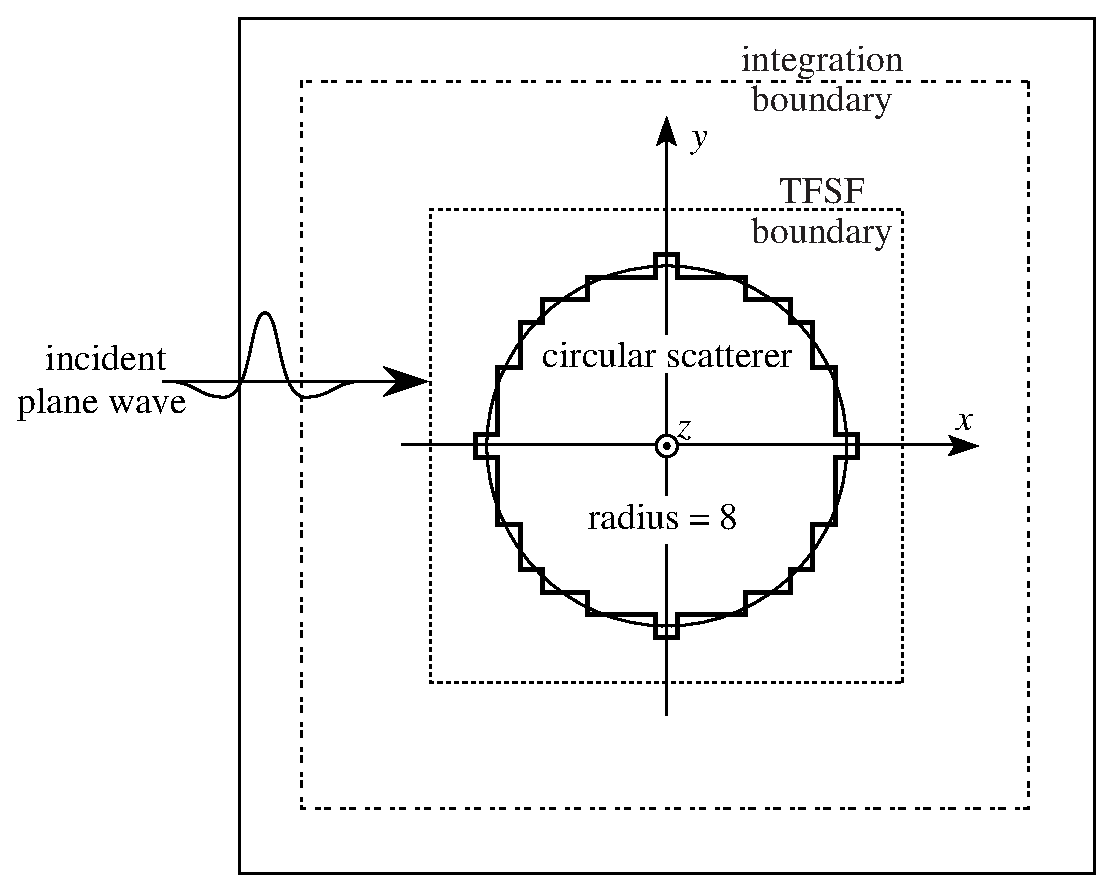
\epsfig{width=4in,file=Figures/Fdtd-near-to-far/cylinderGeom.eps}\\
\caption{Geometry of the circular PEC cylinder.}
\label{fig:cylinderGeom}
\end{figure}

Figure \ref{fig:cylWidth} shows the wavelength-normalized scattering
width of the cylinder as a function of scattering angle obtained using
the series solution for a circular cylinder \cite{balanis1989b}, the
arithmetic-mean NTFF transform, and the GM-NTFF transform.  (The
normalized scattering width is the same as the radiation pattern given
in \refeq{eq:radPattern} where $\rho$ is now taken to be the distance
from the center of the cylinder.)  The discretization is such that
there are $9.92526$ cells per wavelength at the frequency being
considered here.  One should keep in mind that the discretization of
the cylinder introduces some errors and hence the ``exact'' solution
for a circular cylinder is not truly exact for the scatterer present
in the simulation.  Therefore, the reference solution does not provide
a perfect way with which to judge the solutions.  Nevertheless, one
hopes that the FDTD scatterer, when employing the Dey-Mittra scheme,
is a close approximation to a true circular scatterer and thus the
exact solution from the continuous world provides a reasonable basis
for comparison.
\begin{figure}
\begin{center}
\epsfig{width=4in,file=Figures/Fdtd-near-to-far/cylinderWidth.eps}
\end{center}
\caption{Scattering width of a circular cylinder.  The radius is eight
cells and the frequency corresponds to $9.92526$ cells per wavelength.}
\label{fig:cylWidth}
\end{figure}

The difference between the solutions in Fig.\ \ref{fig:cylWidth} are
seen to be relatively small.  Figure \ref{fig:cylErr} shows a plot of
the magnitude of the difference between the exact solution and the 
FDTD-based solutions.  Although there are angles where the arithmetic
mean performs better than the geometric mean, in general the geometric
mean is better.  The integrated error for angles between $0$ and
$\pi$ is $0.6936$ for the arithmetic mean and $0.3221$, i.e., the
error is reduced by more than a factor of two by using the geometric
mean.  
\begin{figure}
\centering
\epsfig{width=4in,file=Figures/Fdtd-near-to-far/cylinderError.eps}\\
\caption{Magnitude of the difference between the FDTD-based solutions
and the nominally exact solution.}
\label{fig:cylErr}
\end{figure}

\subsection{Scattering from a Strongly Forward-Scattering Sphere}

Finally, consider scattering from a dielectric sphere, depicted in
Fig.\ \ref{fig:sphereGeom}, which has a relative permittivity
$\epsilon_r$ of $1.21$.  Such a sphere was considered in
\cite{li2005a2} and can also be found in Sec.\ $8.7$ of
\cite{taflove2005b}.  In this case the transformation traditionally
entails finding the tangential fields over the six sides of a cuboid
which bounds the sphere.  The sphere is discretized such that there
are $60$ cells along the radius.  A staircase representation is used
(where a node is simply either inside or outside the sphere).  The
simulation is run at $95$ percent of the $3$D Courant limit
($0.95/\sqrt{3}$) for $2048$ time steps.  The grid is terminated with
an eight-cell perfectly-matched layer.
\begin{figure}
\centering
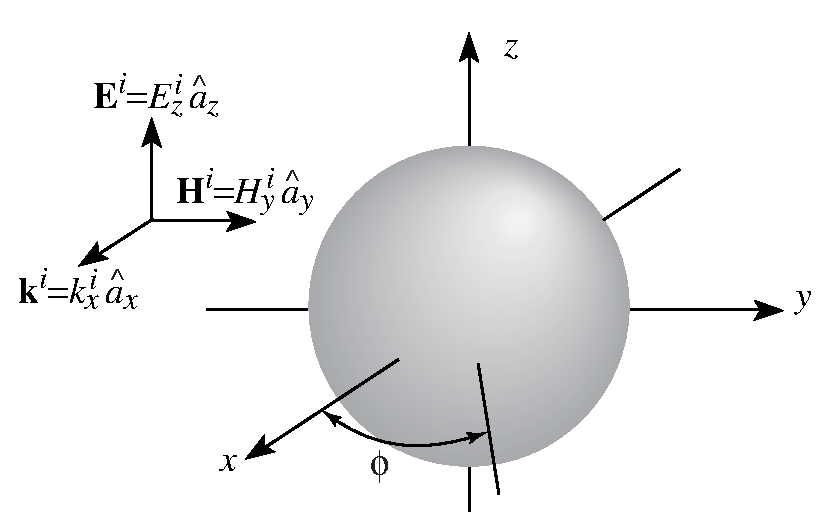
\epsfig{width=4in,file=Figures/Fdtd-near-to-far/sphereGeom.eps}\\
\caption{Geometry of the dielectric sphere.  The relative permittivity
$\epsilon_r$ is $1.21$.  This incident field is polarized in the $z$
direction and travels in the $x$ direction.  The equatorial angle
$\phi$ is in the $xy$-plane with $\phi=0$ corresponding to the $+x$
direction.}
\label{fig:sphereGeom}
\end{figure}

Figure \ref{fig:sphereVsPhi} shows the normalized scattering cross
section as a function of the equatorial angle $\phi$.  The frequency
corresponds to $20.06$ cells per wavelength.  The exact solution was
obtained via the Mie series (see, e.g., \cite{ishimaru1991b}).  As was
the case in $2$D, both the arithmetic and geometric mean perform
reasonably well, but the geometric mean is generally more accurate
than the arithmetic mean.  In Fig.\ \ref{fig:sphereVsPhi} visible
errors are only present near the back-scattering direction of
$\phi=180$ degrees.  Note that there is a large difference,
approximately five orders of magnitude, between the scattering in the
forward and backward directions.  

\begin{figure}
\centering
\epsfig{width=5.4in,file=Figures/Fdtd-near-to-far/cross-section-vs-phi.eps}\\
\caption{Scattering cross section of a dielectric sphere versus the
equatorial angle $\phi$.  The sphere is discretized with $60$ cells
along the radius and the frequency used here corresponds to $20.06$
cells per wavelength.}
\label{fig:sphereVsPhi}
\end{figure}

In order to improve the results in the back-scattering direction Li
{\em et al.}\ \cite{li2005a2} advocated calculating the transformation
using the five faces other than the forward-scattering face.  Figure
\ref{fig:sphereBackscatterArith} shows the normalized backscattering
cross section versus wavelength (expressed in terms of number of cells
per wavelength) calculated using the arithmetic mean.  The normalized
cross section is given by
\begin{equation}
  \frac{1}{\lambda^2}\lim_{r\rightarrow\infty}
   \left[4\pi r^2\frac{|\hat{E}_z(\theta,\phi)|^2}{|\hat{E}_z^i|^2}\right]
  \label{eq:crossSection}
\end{equation}
where $r$ is the distance from the center of the sphere, $\theta$ is
the azimuthal angle and $\phi$ is the equatorial angle.  For
backscatter, $\theta$ is $\pi/2$ and $\phi$ is $\pi$.

The NTFF transform results shown in Fig.\
\ref{fig:sphereBackscatterArith} were calculated using either the
fields over all six faces of the integration boundary or the fields
over the five faces advocated by Li {\em et al.}  The results in this
figure correspond to those shown in Fig.\ 1(b) of \cite{li2005a2} for
the sphere with a radius of $3$ $\mu$m.  (However, for the sake of
generality, here the results are plotted in terms of unitless
quantities.)  Note that the six-sided arithmetic-mean results
presented here are better than those presented in \cite{li2005a2}.  We
were able to duplicate the results presented in \cite{li2005a2} by not
applying a temporal phase-correction factor (or, similarly, by
applying a correction factor which is twice the factor given here).
Nevertheless, the recommendation of Li {\em et al.}\ is true that the
five-sided computation is better than the six-sided one for
calculating the backscattering when using the arithmetic mean.
However, for directions other than backscatter or for other sizes, one
does not know {\em a priori} if a face should or should not be
discarded.

\begin{figure}
\centering
\epsfig{width=5.4in,file=Figures/Fdtd-near-to-far/back-arithmetic.eps}\\
\caption{Backscatter from a sphere with $\epsilon_r=1.21$ versus the
wavelength (expressed in terms of number of cells).  The FDTD
transformations are calculated using the arithmetic mean and either
a five- or six-sided transformation boundary.}
\label{fig:sphereBackscatterArith}
\end{figure}

Figure \ref{fig:sphereBackscatterGeom} is the same as Fig.\
\ref{fig:sphereBackscatterArith} except the transformation is done
using the GM-NTFF transform.  In this case discarding data from the
forward-scattering face actually slightly degrades the quality of the
transform.  Thus, when using the geometric mean there is no need to
discard data.  One can use it confidently for all scattering angles
and all sizes.

\begin{figure}
\centering
\epsfig{width=5.4in,file=Figures/Fdtd-near-to-far/back-geometric.eps}\\
\caption{Backscatter from a sphere with $\epsilon_r=1.21$ versus the
wavelength (expressed in terms of number of cells).  The
transformations use the geometric mean and the fields over either five
or six faces of the integration boundary.}
\label{fig:sphereBackscatterGeom}
\end{figure}

To summarize, unlike the traditional arithmetic mean, for a single
harmonic plane wave the geometric mean accounts for the spatial offset
of the fields in a way that is exact.  In practice, where a spectrum
of wave vectors are present, the geometric mean typically performs
significantly better than the arithmetic mean.  The geometric mean is
much less sensitive to the integration-boundary location than is the
arithmetic mean.  For strongly forward-scattering objects, the use of
the geometric mean obviates the need to discard the fields over the
forward face (as has been advocated previously) when calculating the
backscatter.  The geometric mean does entail a slight increase in
computational cost because for each node along the integration
boundary a DFT must be calculated for three fields instead of two.
However, this cost is typically minor compared to the overall
simulation cost.

